\documentclass{sig-semester}

\pdfpageheight=11in
\pdfpagewidth=8.5in

\usepackage{latexsym}
\usepackage{amsmath}
\usepackage{amssymb}
\usepackage{color}
\usepackage{enumerate}
\usepackage{graphicx}
\usepackage{amssymb}
\usepackage{epstopdf}
\usepackage{xspace}

% These are from candidacy edic.tex
\graphicspath{{./graphics/}}
\DeclareGraphicsExtensions{.pdf,.jpeg,.png}

% Legacy from Christoph's paper:
% \DeclareGraphicsRule{.tif}{png}{.png}{`convert #1 `dirname #1`/`basename #1 .tif`.png}

% When converting eps to pdf, suffix is added to filename. 
% Recommended not to be empty string by http://www.tex.ac.uk/tex-archive/macros/latex/contrib/oberdiek/epstopdf.pdf : page 4, suffix paragraph.
\epstopdfsetup{suffix=-generated}

\newtheorem{theorem}{Theorem}[section]
\newtheorem{proposition}[theorem]{Proposition}
\newtheorem{example}[theorem]{Example}
\newtheorem{remark}[theorem]{Remark}
\newtheorem{todo}[theorem]{ToDo}
\newtheorem{algorithm}[theorem]{Algorithm}
\newtheorem{metatheorem}{Metatheorem}[section]
\newtheorem{definition}[theorem]{Definition}
\newtheorem{property}[theorem]{Property}
\newtheorem{corollary}[theorem]{Corollary}
% \newtheorem{lemma}[theorem]{Lemma}
\newtheorem{conjecture}[theorem]{Conjecture}
\newtheorem{proviso}[theorem]{Proviso}


\title{Cumulus: Decentralized Data-Parallel Online Aggregation by Message Passing}


%\numberofauthors{1}
\author{\alignauthor Aleksandar Vitorovic \\[1ex]
\affaddr{Dept.\ of Computer Science} \\
\affaddr{EPFL} \\
\affaddr{aleksandar.vitorovic@epfl.ch}
}

\def\M3{M3\xspace}
\def\EXORD{actual update execution order\xspace}

\hyphenation{decla-rative speci-fies signifi-cantly atomici-ty}

\begin{document}
\maketitle


\abstract{
We present Cumulus, a distributed data-parallel online aggregation system.
Cumulus compiles a set of SQL aggregation queries
down to a message-passing program that incrementally maintains
the query results by simple and highly efficient local modifications.
Surprisingly, our message passing programs
perform only a {\em constant}\/ amount of work
for each tuple inserted or deleted and each
aggregate value to be maintained.
Our message-passing protocol allows for massive parallelization.

The Cumulus runtime system is a distributed key-value store for
aggregate-group-by query results that implements our message passing protocol
for incremental result maintenance. 
Cumulus uses the resources of the cloud to leverage parallelism 
and keep its store in main memory.
We ensure serializability without synchronization.
Cumulus is able to perform the incremental maintenance of
large views under considerable update loads in realtime.\\
}


\keywords{Incremental View Maintenance, updates, Parallelization}


\section{Introduction}
\vspace{2mm}

Recent years have seen the beginning of a paradigm shift in data management research from incrementally improving decade-old database technology to questioning established architectures  and creating fundamentally different, more lightweight systems that are often domain-specific (e.g.,
\cite{DBLP:conf/vldb/StonebrakerMAHHH07,DBLP:journals/pvldb/KallmanKNPRZJMSZHA08}).

Part of the impetus for this change was given by potential users such as scientists and the builders of large-scale Web sites and services such as Google, Amazon, and Ebay, who have a need for data management systems but have found current databases not to scale. One can observe a trend to disregard database contributions in these communities \cite{dbcolumn, DBLP:conf/sigmod/PavloPRADMS09}, and to build lightweight systems based on robust technologies, mostly pioneered by the operating systems and distributed systems communities, such as large scale file systems, key-value stores, and map-reduce \cite{DBLP:journals/cacm/DeanG08, DBLP:journals/tocs/ChangDGHWBCFG08}. Further impetus has resulted from the current need to develop data management technology for multicore and cloud computing.

There is a recent tendency among pundits outside the database community to contest the need for powerful queries, and to think of distributed key-value stores (maps) -- with only the power to look up data by keys -- as (much more efficient) database query engines. However, expressive query languages such as SQL continue to act as an important intermediary between users and more complex data-processing tasks. 

This paper brings SQL expressiveness along with efficiency od distributed key-value store. Using DBToaster \cite{SQLCompiler09}, an aggressive recursive incremental view maintenance compiler, SQL is translated to a trigger-based vector processing language, called \M3. 

In most traditional database query processors, the basic building blocks of queries are large-grained operators such as joins. Conversely, a large class of SQL aggregation queries can be compiled down to very simple, extremely efficient message passing C++ programs that incrementally maintain materialized views of the queries. Using Incremental View Maintenance \cite{Lee01}, the complexity of query response times can be substantially reduced. Yet, by applying incremental view maintenance recursively, the complexity of query response times is trimmed down to constant time, for a limited set of queries.

These \M3 message passing programs keep a hierarchy of map data structures (which may be served out of a key-value store) up to date. They can share computation in the case that multiple aggregation queries (e.g., a data cube \cite{datacube}) need to be maintained.  Most importantly, though, these message passing programs can be massively parallelized to the degree that the updating of each single result aggregate value can be done in constant time on normal off-the-shelf computers\footnote{Note that since there are usually many more aggregate values to maintain than there are processors,
this does not mean that each update is processed in constant time.}. This is proven in the Koch's Algebra paper \cite{KochAlgebra10}, in the case when polynomial amount of hardware and space is available.

\M3 programs are interpreted within our runtime system, Cumulus. The Cumulus is a thin execution layer that lives above generic key-value stores and implements the message passing protocol. It can efficiently process a wide range of incremental view queries. The query results are stored in the distributed key-value store itself, as ordinary data.

Cumulus is a multiversion timestamp-based concurrency control system running in a shared-nothing main-memory environment. The maps are distributed among processing nodes, and a user may submit an update just as the data was local. Out-of-order execution of updates are fully supported, and if there are violated dependencies, additional messages, called corrective update messages, are sent.

Cumulus is built around a novel hybrid consistency execution framework. Like most cloud data management systems, Cumulus achieves low latencies by retreating to the realm of eventual consistency. However, unlike most eventual consistency systems, Cumulus' runtime periodically generates consistent snapshots as a side effect of its normal operation. The result is a system that can be employed side-by-side by both applications that require low latency and applications that require strong consistency.

We believe that our contribution constitutes an important step towards achieving the apparent contradiction in terms of executing complex aggregation queries on updateable data using a little more than a distributed key-value store.

The next section present system overview and requirements, in the context of \M3 programs generated by DBToaster. Section~\ref{sec:sysdesign} presents the message passing protocol guiding reader through existing data dependencies and logical components in the system, further explaining consistency achieved and possible optimizations. In Section~\ref{sec:Experiments}, the experiments performed and its results are explained, while Section~\ref{sec:Related} contains related work. Section~\ref{sec:Future} presents possible future improvements of the system, while Section~\ref{sec:Conclusion} coalesces all the ideas grasped from the work.

\section{System overview \& requirements}
\vspace{2mm}

A user would like efficiency of C programs, while declarative nature of SQL. The gap will be shrunk by introducing \M3 compiler which compiles updates to C language constructs \cite{DBToasterCompiler09}. \M3 compiler will generate \M3 trigger program to cover all the updates in the system. An update (event) refers to an incremental change of a relation, i.e. an insert or delete of a tuple. A tuple modification is implemented as a delete followed by an insert. A trigger is coupled with arguments, which represent tuple fields necessary for an update. Cumulus takes a compiled program as the input, and on each update arrival executes a trigger program with the corresponding arguments. In general, Cumulus is a system designed for providing realtime answers to OLAP aggregation queries in an environment where OLTP updates are continuously arriving.

\begin{example} \em
\label{ex:simpleTrigger}
An insert trigger and its possible instantiation (update):
\begin{verbatim}
ON +R(A,B){
   m1+=m2[A];
   m2[A]+=m3[B];
}
ON +R(10,20){
   m1+=m2[10];
   m2[10]+=m3[20];
} 
\end{verbatim}
\end{example}
The corresponding delete trigger is the same, except there is always a multiplication with -1 on the right hand side.

\textbf{Data structures.} The only data structures used by transition programs are maps. A map contains a unique name and a pair \{key, value\}. Multikeyed pairs are supported as well. A map reference contains only a map name and a key(s). A map collection consists of a map name and the key/value pairs from the whole domain of keys. In comparison with the classical database containers, a map refers to a relation or an intermediate result, whereas a key(s) represents a position in a relation.

A trigger consists of multiple statements which perform operations on maps. An \M3 program reads maps from the right-hand side, and writes to the left-hand side map of the statement. The map name and the trigger arguments specifies a map to be accessed. If a variable used in a statement in a trigger is not defined in the trigger arguments, the whole map domain participates in the statement. On the right-hand side of the statement, the only allowed operation is multiplication, while between left and right side only += is permitted. Thus, each statement adds a \textit{delta} to the left-hand side map. Initially, map collections are empty. If a read or write operation is performed on a non-initialized map, zero is assumed.

DBToaster generates only acyclic map data dependencies flow graph \M3 programs. In runtime, execution of \M3 programs must provide the following guaranties:
\begin{itemize}
 \item Updates execute atomically with respect to each other. The effect has to be the same as whole update sequence was processed sequentially.
 \item Statements within same update use right-hand side maps from the state of the system right before current update start executing.
\end{itemize}

An update stream (i.e. ticker feeds, sensors, static files, relational databases, or even other \M3 programs) continuously injects events (triggers instantiated with arguments). The aim of our system is to process those updates and add deltas to the appropriate maps.

As there is a large amount of data, maps should be distributed among many processing nodes. The only way processing nodes could communicate is via sending and receiving messages. In order to achieve constant execution time complexity and support embarrassing parallelism, the protocol for sending/receiving messages has to avoid complex map locking schemes and support simultaneous map updates.

Also, our system has to be tolerant to reordering of messages which occurs in large networks. We assume the network supports pairwise in-order delivery, but different processing nodes may observe different order of messages arrived from the multiple processing nodes. Our system may only rely on the property that every sent message will eventually arrive to its destination; messages cannot be lost in the network.

Delay is another network characteristic which may significantly degrade overall performance. Only one message sent to all other nodes in a 10.000 processing node system will effect in delay for several seconds. Therefore, it is extremely important to build protocol based on the lowest possible number of exchanged messages.
 
Different queries will have different materialized view and will operate on different maps, supporting parallelism inherently. Our goal is to parallelize updates relevant to one complex SQL query a user is interested in. That way, not just throughput, but also latency could enhance.

All data will be stored in main memory in order to achieve better performance. 
We generally assume that the data is persistent in the OLTP databases.
However, our system is also able to
log update streams and replay it from the
log later to recreate the data warehouse in main memory.
We could also log the map states using techniques as surveyed in
\cite{DBLP:journals/pvldb/SallesCSDGKW09}
for faster recovery, but this is currently not done.

\section{System design}
\label{sec:sysdesign}
\vspace{2mm}

\subsection{Data Dependencies}
In this section, we will present types of dependencies, and how they could be violated, while Section~\ref{Corrective} presents the structures used for avoiding dependency violations.

There exists three types of dependencies corresponding to different statements \texttt{STMT1} and \texttt{STMT2}:
\begin{itemize}
 \item \texttt{Write-Read}: \texttt{STMT2} is later in an update stream and reads from a map that \texttt{STMT1} writes to
 \item \texttt{Read-Write}: \texttt{STMT2} is later in an update stream and writes to a map that \texttt{STMT1} reads from
 \item \texttt{Write-Write}: Both \texttt{STMT1} and \texttt{STMT2} update the same map
\end{itemize}

Write-Write dependency violation may occur even within a single update. Write-Read and Read-Write dependencies within the same update could not be violated because, according to \M3 program guaranties, no map read will return the value from the current update. Therefore, we imply logical order between statements, based on Timestamps of the update a statement belongs to. In case of a single update stream, Timestamp (TS) is a implicitly defined unique serial number of an update in that update stream. For multiple update streams, some total order has to be introduced. An Introduced Total Order among all the updates is achieved by expanding TS with update stream ID, thus forming <TS, update-stream-id> pairs. TS preserves order of updates arrived from a single update stream, while update-stream-id breaks ties among updates with the same TS. The update stream ID may be generated statically or by utilizing the Standard Renaming Technique \cite{Welch04}.

Introduced Total Order is different from happened-before relation defined in \cite{Lamport78}. Data dependencies may exist between events from multiple input streams, and has to be preserved. If two events in Introduced Total Order have data-dependencies, the event with smaller TS \textit{logically precedes} or \textit{is prior to} the other one, while the event with higher TS \textit{logically succeeds} the other one.

Consider an example shown in Figure~\ref{fig:streamWR}. For the Introduced Total Order, a Write-Read dependency exists on m2[1] between the second statement in the first update and the first statement in the second update.

\begin{figure}
\begin{center}

\begin{tabular}{c|c|r}
TS & Update & Statement\\
\hline
1 & ON +R(1,4) & m1 += m2[1]    \\
  &            & m2[1] += m3[4] \\
\hline
2 & ON +R(1,5) & m1 += m2[1]    \\
  &            & m2[1] += m3[5] \\
\end{tabular}
\end{center}

\vspace{-3mm}
\caption{W-R on m2[1] for Example~\ref{ex:simpleTrigger}.}
\label{fig:streamWR}
\vspace{-2mm}
\end{figure}



\begin{example} \em
\label{ex:foreachTrigger}
Consider the following insert triggers and a sequence of updates:
\begin{verbatim}
ON +R(A){
   m3[C]+=m1[A]*m2[C];
}
ON +S(B){
   m2[B]+=1;
}

TS1: ON +R(1)
TS2: ON +S(2)
\end{verbatim}
\end{example}

Since the variable C in the \texttt{+R(A)} trigger is not present in the trigger arguments, loop over whole m3 domain is implied. If statements from \texttt{+R(A)} and \texttt{+R(B)} are performed on different processing nodes, the update from TS2 may complete before the update from TS1 read m2[2] value. Thus, Read-Write dependencies are violated.

In addition, an update should be processed atomically. The result of update has to be the same as all statements inside an update were executed at the same point in the time. In other words, all updates have to be executed in some total order.

\begin{example} \em
\label{ex:mulInput}
Atomicity could be violated in
\begin{verbatim}
ON +S(A){
   m1[A]+=m2[A]
}
ON +T(B){
   m2[B]+=m1[B];
}\end{verbatim}
when the following update sequence emerges:
\begin{verbatim}
 S(1)
 T(1)
\end{verbatim}
\end{example}
The necessary conditions are:
\begin{itemize}
 \item For the update sequence, statements from \texttt{+S(A)} and \texttt{+T(A)} are performed on different processing nodes.
 \item Both updates synchronously read map on the right side then synchronously write to map on the left side. 
\end{itemize}

Note that atomicity can not be violated by writing to a single map as all the processing on a single processing node is done sequentially.

Even if atomicity is preserved, Introduced Total Order may differ from \EXORD. For example, if Introduced Total Order was \texttt{S(1), T(1)} and \EXORD was \texttt{T(1), S(1)}, both the Read-Write and the Write-Read dependencies are violated.

\subsection{System components}
\label{Components}
\vspace{2mm}

Overall system architecture is presented in Figure~\ref{fig:architecture}. There are two logical components in the system.
\textit{Switches} maintains information about map partitioning and, by sending messages, delegate map updates from update streams to a number of data storage and query processing nodes, or \textit{Data Warehouse (DW) Nodes}. The DW Nodes store maps and perform computations on them. The \textit{client} sends queries which will probe the system and return a requested set of maps. Separate messages have to be sent between a pair of processing nodes, as multicast is not efficient, and in cloud computing not supported at all. In the further text, by updates we assume events in the system, whereas map updates are always denoted fully.

\begin{figure}
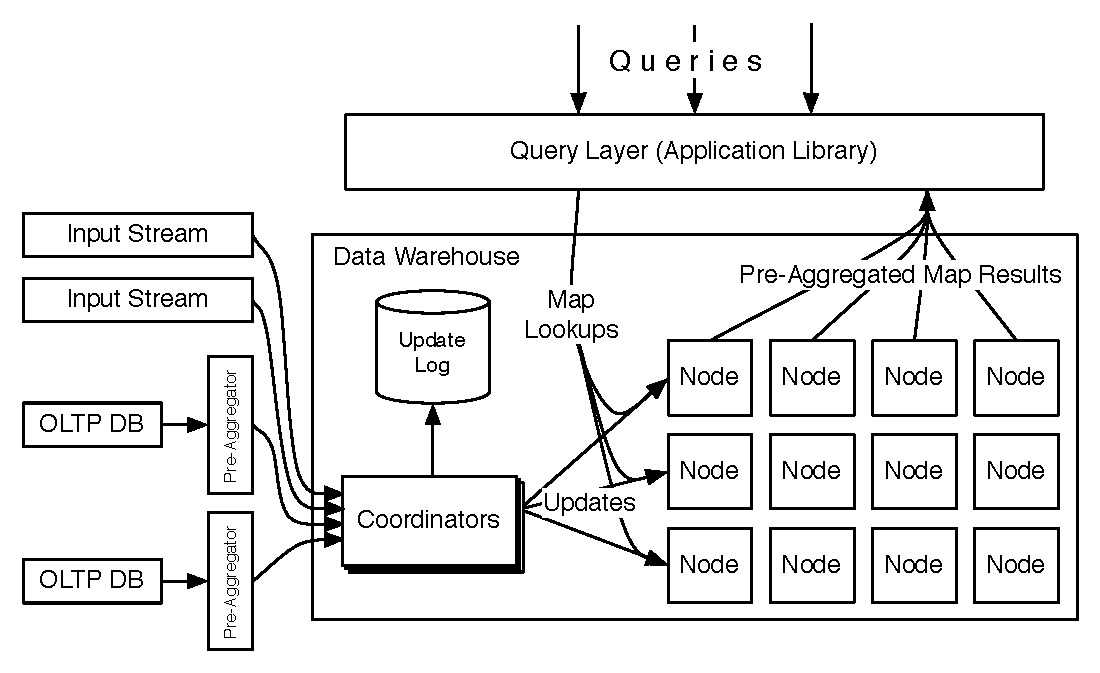
\includegraphics[width=3in]{Architecture.pdf}
\vspace{-3mm}
\caption{System Architecture}
\label{fig:architecture}
\vspace{-2mm}
\end{figure}

Due to the in-order delivery between any two nodes, using only one switch simplifies the system design as arriving updates are implicitly serialized. Thus, violations of data dependencies are sidestepped. On the other hand, single-switch system implies some serious performance limitations. Firstly, the switch will be bottleneck, so the system does not scale. Secondly, a single point of failure property will exist in the system by design. Therefore, our system will contain several switches, i.e. one switch per update stream.

Each statement in an update employs three classes of actors:
\begin{itemize}
 \item Source nodes: The nodes hosting the right-hand side maps.
 \item Computation nodes: The nodes where statements are evaluated.
 \item Destination nodes: The nodes hosting the left-hand side map.
\end{itemize}

\begin{figure}[!b]
\begin{center}
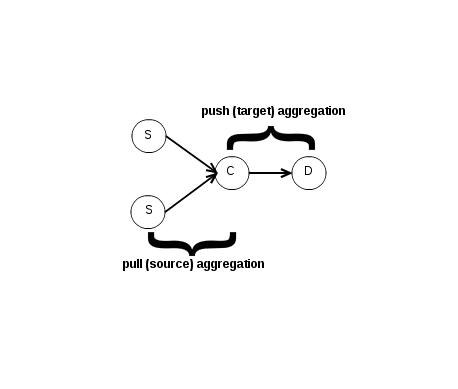
\includegraphics[width=2in]{pushPull.jpg}
\vspace{-3mm}
\caption{Push and pull aggregation}
\label{fig:pushPull}
\vspace{-2mm}
\end{center}
\end{figure}

Assume we have a statement m+=m1[a]*m2[b]. We need to identify the sources (at most two DW Nodes), to compute the result and store the result to the destination. Those actors are logical entities: it is not necessary (and in fact, typically detrimental) for the actors to be on separate physical nodes within the cluster. The system may employ different mappings of logical DW Nodes distribution (source, computation, destination) across physical hardware in the cluster for each invocation of each statement.

\textbf{Destination-computation.}
Co-locate the processing of an \M3 statement (the computation nodes) with the DW Node storing the left-hand side map (the destination node). Each source node transmits all relevant maps to the destination node. Upon arrival, the destination node evaluates the statement and stores the result.

\textbf{Source-computation.} Instead of processing map updates at the DW Node where the result will be stored (the destination node), precompilation allows our system to ensure that all data necessary to process a statement is co-located. Rather than storing the results locally, a replica of the map is created at each DW Node that reads from the map. When evaluating an map update, the computation can be performed instantaneously.

However, it is typically not possible to generate a partitioning of the data that ensures that for each statement in a \M3 program, all the source nodes will be co-located. Due to replication, our system may have multiple destination nodes, so the overhead of transmitting the result to the destination nodes is introduced. While replication is typically a desirable characteristic, storage-constraint infrastructures may need to use complex partitioning schemes. Thus, our system will use destination-computation approach.

Figure~\ref{fig:pushPull} presents both Destination-computation and Source-computation approaches.

A set of messages issued by a switch for destination-computation approach is illustrated in Figure~\ref{fig:msgs}. FETCH messages are sent to DW Nodes that contain the right-hand side maps. In the further text such DW Node will be denoted as the DW Read Node, by role they play in current statement. The DW Read Node will send PUSH message containing the data read to the DW Node that contain the left-hand side map. In the further text such DW Node will be denoted as the DW Write Node, again, by role they play in current statement. Same DW Node may be the DW Write Node for one statement and the DW Read Node for some other statement. The DW Write Node will be aware of the map update to perform by receiving PUT message from a switch. For each statement, there is exactly one PUT message (since only one map can be the left-hand side) and one or more FETCH/PUSH messages (since there may exist multiple source nodes).

\begin{figure}
\begin{center}
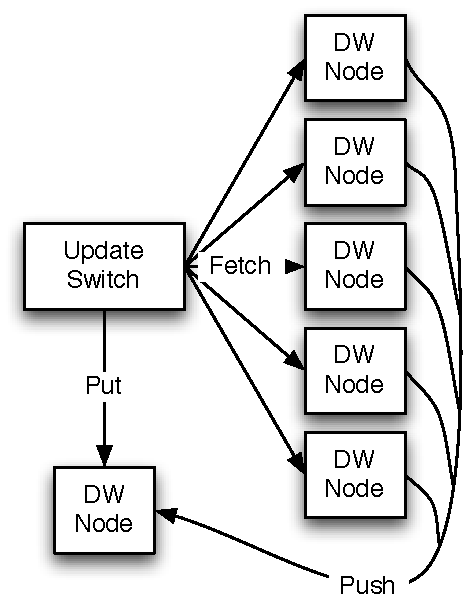
\includegraphics[width=1.5in]{UpdateStep.pdf}
\vspace{-3mm}
\caption{Messages between a switch and a DW Node}
\label{fig:msgs}
\vspace{-9mm}
\end{center}
\end{figure}

The content of the messages in the system will be shown on the first statement in Example~\ref{ex:simpleTrigger}. In order to reduce the network traffic to a minimum, a switch need not to send to a DW Node all the operations that will be applied on the maps. If each DW Node contains current \M3 program, a switch may send to a DW Write Node only a unique ID of the statement. The ID of the statement could simply be a line number in a file which contains all statements in \M3 program.

The system could coalesce all messages with the same source, destination and TS into a single one. Multiple FETCH messages per TS may be sent only if there are multiple DW Read Nodes per update, similarly, multiple PUT messages per TS may be sent only if there are multiple DW Write Nodes per update. For all types of messages, since DW Nodes are aware of current \M3 program and its triggers, a unique ID of trigger, instead of a unique ID of statement, is sent. Thus, the message traffic is significantly reduced. In addition, single message per Timestamp forbids outside world to see Timestamp-inconsistent version of the map (i.e. two same left-hand side maps are updated withing single update and result of the first one is visible to the outside world).

A switch will send a FETCH message to each DW Read Node containing some of the right-hand maps (in our example to a single DW Read Node containing m2[10]) with the following encapsulated information:
\begin{itemize}
 \item Trigger ID
 \item Trigger arguments relevant to the DW Read Node
 \item TS of the update
 \item A reference to a DW Write Node (in our example the DW Node containing m1)
\end{itemize}

A DW Read Node can extract information which maps to send from Trigger ID. A DW Read Node will check all the right-hand side maps from the update, and send each of them which is stored on current DW Read Node in a single PUSH message to the all relevant DW Write Nodes.

A DW Read Node sends a PUSH message to the DW Write Node with the following encapsulated information:
\begin{itemize}
 \item Trigger ID
 \item TS of the update
 \item A list of the right-hand side maps from the DW Read Node (in our example m2[10])
\end{itemize}

A switch will send a PUT message to the DW Write Node with the following encapsulated information:
\begin{itemize}
 \item Trigger ID
 \item Trigger arguments relevant to the DW Write Node
 \item TS of the update
\end{itemize}

A DW Write Node could match a PUSH message with a corresponding PUT message by TS. A DW Write Node could not complete processing a PUT message until the PUSH messages from all corresponding DW Read Nodes arrived. For each statement within a trigger, the DW Write Node will compute the right-hand side of a statement and add computed value to the left-hand side map. Note that even non-initialized maps must be initialized to zero and sent; the DW Write Node needs to hear from all DW Read Nodes in order to proceed with its write.

The DW Node utilizes the \textit{ReceiveLog} and a list of boolean flags per statement for matching PUT and PUSH messages. The ReceiveLog, consisting of pairs \{map, TS\}, is responsible for storing all maps from the PUSH messages. When a PUT message arrives, the DW Write Node will initialize the lists of boolean flags for each statement in the update the PUT message refers to. Each arrived PUSH message will append ReceiveLog and set appropriate boolean flag for the corresponding PUT message. (It may happen to have multiple boolean flags across update if the arrived map is appearing in multiple right-hand side maps.) If some PUSH message arrives before the corresponding PUT message, a list of boolean flags may be initialized, utilizing Trigger ID from the message. From arrival of the PUT message to the time when all necessary boolean flags are set, processing the PUT message is suspended, so other messages may arrive (including awaited PUSH messages). Until completing PUT message processing, no messages with higher TS is processed, in order to prevent data dependency violation.

Upon all necessary boolean flags are set for a statement, map update is performed, using accumulator. Since the only operation on the right-hand side is multiplication, the accumulator will set its initial value to 1. Then, the value from accumulator is multiplied with each the right-hand side map, and again stored in accumulator, until all of them is processed. Finally, += operation between the left-hand side map and accumulator is performed.

A client could obtain some query answer from our system by sending queries to a switch. A switch will issue a QUERY message encoded, among with TS and the reference to the switch a client is communicating with. After receiving the maps from the DW Nodes, the switch will submit them to the client. Alternatively, a client may access the DW Nodes directly, using a map partitioning information obtained from a switch.

If we assume partitioning is static, information about map distribution could be sent to all DW Nodes before any update arrived. Thus, the FETCH messages need not to contain relevant DW Write Node information, providing additional message traffic reduction.

\subsection{Corrective updates}
\label{Corrective}
In this subsection, steps taken upon dependency violation is presented. 

The corrective mechanism is an implementation of apologies in ``memories, guesses and apologies`` mechanism mentioned in \cite{helland09}. Multiversioning, along with the corrective update mechanism, provides virtual synchrony \cite{Birman87a}. That is, DW Nodes run \M3 code in parallel without enforcing lock-step, but still providing enough guaranties as when lock-step is present. The corrective update mechanism is the key for achieving the goal.

As already mentioned, Introduced Total Order may not reflect \EXORD. A statement on a DW Node sees only the effects of prior statements, though it may not see all of them, thus potentially violating dependencies. A DW Node itself cannot be aware whether some update will arrive later due to processing on a slow switch and/or network delays, or will never arrive since it is irrelevant to our DW Node (no maps stored in our DW Node in particular TS).

Our system uses an optimistic approach, continue whenever possible, and if some dependencies are violated, employ the \textit{corrective update} mechanism. Since our computation is based on delta processing, work done speculatively need not be thrown away entirely. Rather, any work done can be revised though deltas, to the final desired outcome. However, out-of-order events are expected to occur infrequently. Furthermore, such events are likely to interfere only a handful of prior updates, for example a write on one map followed by an out-of-order read on a different map does not cause a problem. Since increasing number of switches and/or update streams yields more messages in the system, there is higher probability for delays and reordering of messages, violated data dependencies and finally, corrective update messages.

Our system could recognize dependency violation by combining information about maps sent and received along with their TS. For that purpose, we will take a look at a simple statement mw+=mr. Assume the DW Read Node contains mr, while the DW Write Node contains mw. All information about sent map are presented in the mr(TSx, TSy) notation. There are three types of dependencies, we will tackle them separately:

\begin{itemize} 
 \item \texttt{Read-Write}:  If at the DW Write Node, after applying write in TSy, arrive a FETCH message referring to mw with TSz such that $z<y$, the DW Write Node will send some previous version of mw.

 \item \texttt{Write-Write}: If at the DW Write Node, after applying Write on TSy, arrive a PUT message referring to mw with TSz such that $z<y$, both versions of mw could still be needed, depending of future arrival of messages and their TS. Since there is only one PUT message per DW Write Node in an update, Write-Write dependencies could not be violated within the single Timestamp.
 
 \item \texttt{Write-Read}:  If at the DW Read Node, after sending mr, arrive a PUT message referring to mr with TSz such that $z<y$, Write-Read dependency is violated. At the time of sending mr, the DW Read Node can not be aware whether the sent map is consistent, or the PUT message with TSz will arrive later due to the network delays. Thus, the DW Read Node optimistically send the most recent version of the map prior to TSy. However, when the PUT message with TSz arrives, the DW Read Node has to send the delta applied to mr in TSz. The message containing the delta is denoted as the \textit{corrective update} message.

\end{itemize}

Since the only operation on the lhs is adding deltas, writes to the same map can be applied in any order, as long as others receive correct version (or a delta in the Write-Read case).

The goal is is to ensure that a processing node never has to wait to read a map, therefore multiple versions of each map is maintained, each with a TS. Therefore, the \textit{WriteLog} structure, consisting of pairs \{map, TS\}, is exploited. Thus, Write-Write dependencies could not be violated, while violating Read-Write dependencies is avoided by reading the most recent version of the map prior to the Read TS. For preserving Write-Read dependencies, the WriteLog is also used, but a delta from versions of the map is extracted. On the DW Read Node side, upon receiving a PUT message referring to map mr with TSz, corrective updates will be sent to each DW Write Node which used map mr as right-hand side map for their computation in TSy such that $z<y$. The \textit{ReadLog} structure will maintain pairs \{map reference, reference to DW Write Node, TSy\}, so our system could iterate over this structure exploring the entries fulfilling the condition.

Note that the pairs from the ReceiveLog and the WriteLog are the same. The only difference is that the WriteLog maintains history of the maps on the current DW Node, while the ReceiveLog maintains history of the maps from the other DW Nodes. In addition, the ReadLog will be utilized even if the right-hand side map and the right-hand side map are on the same DW Write Node, since Write-Read dependencies may be violated even on a single DW Node (i.e. messages regarding different TS arrived from different switches out-of-order).

Corrective update message is similar to a PUSH message, but with different TS. It consist of:
\begin{itemize}
 \item TSx of the last right-hand side map update on the DW Read Node (last mr update in our example)
 \item A delta of the right-hand side map (the delta of mr in our example)
\end{itemize}

Note that the PUSH message contains TSy, while TSx is utilized for corrective update messages. PUSH message refers to exactly one Timestamp on the DW Write Node, while corrective update has to be applied on each update which logically succeeds TSx and use map from corrective update message.

Upon arrival, all types of messages on a DW Node, including FETCH, PUSH, PUT and corrective messages, are stored in the same prioritized buffer by their TS. Thus, the frequency of corrective updates will be amortized.

At the time of processing of corrective update message on the DW Write Node, the following steps have to be taken:
\begin{enumerate}[(1)]
 \item Update all the mr in the ReceiveLog which logically succeeds TSx.

 \item For each map update performed on current DW Write Node that logically succeeds TSx, if mr was used as the right-hand side map, apply map update to each affected pair \{mw, TSy\} in the WriteLog structure. In order to support this, DW Node log all updates (TS, trigger and trigger arguments) in which it performed any read/write operation in the \textit{OperationLog}. The result of a multiplication between the delta on the arrived map and the values of all the remaining right-hand side maps from the ReceiveLog, is added to affected mw. If the delta is applied to a pair \{mw, TSy\}, it has to be applied to each mw in the WriteLog structure succeeding TSy. This is due to implicit Write-Read dependencies between any two += operations with the same left-hand side map.

 \item Corrective updates could be recursive, since the DW Write Node could propagate incorrect mw further to the DW Write Nodes that used mw as the right-hand side map. For each map reference in the ReadLog concerning mw which logically succeeds TSy, corrective update mechanism is applied recursively, but on the \{mw, TSy\} pair.
\end{enumerate}

The recursive mechanism will be more efficient if all mw maps on the local DW Node is firstly updated.

Since corrective update refers to a map which already exist in the ReadLog, the corrective updates will never create new entry in the ReadLog. Furthermore, there is no need for maintaining complete history of maps in the ReadLog, yet only to have highest TSy for each pair \{map reference, reference to DW Write Node\}. A value $y$ may only increase, and if for some arrived corrective update with TSz such that $z<y$, it will hold after $y$ increased. The ReadLog structure do not store information about last map update for which corrective update was sent, yet for the highest TS of sent map.

We will show now that corrective update mechanism terminates. Due to the finite size of each event, a finite number of PUT messages will arrive out of order to a DW Read Node. On a DW Write Node, a finite number of corrective messages will arrive and a finite number of recursive corrective updates will be sent. Since data flow graphs are always acyclic, recursive corrective updates are bounded by the maximum path length in the data flow graph. The acyclicity comes from the fact that some total order was introduced, so a DW Node may send corrective update only to a DW Node which executed event with higher TS. Thus, corrective updates will eventually terminate and all the maps will eventually achieve correct value.
 
On Figure~\ref{fig:correct}, an enhanced example of out of order execution is presented. Messages in the same line are simultaneous, and arrive before messages from next line. Their logical ordering is specified in parenthesis in the figure. The DW Read Node stores map mr, which is used as the right-hand side map in computations of mw on the DW Write Node. Both PUT and FETCH messages on the DW Read Node corresponds to mr, while PUT messages on the DW Write Node corresponds to mw. For the PUT messages on the DW Read Node there is no corresponding FETCH messages, since mr+=1. Assume PUT(TS10) on the DW Read Node comes before TS7 on both DW Nodes, as depicted in the figure. The WriteLog of the DW Read Node is employed, and the most recent mr with TS less than 7 is sent (in this case value from TS2). The same value will be sent for PUT(TS9). However, for PUT(TS11), mr value from TS10 will be sent. In our example PUT(TS6) may arrive later, so it is time to exploit the ReadLog structure. Corrective update will be sent to all DW Nodes which demanded mr with TS greater than 6 (in this case including DW Write Node). Note that the DW Write Node could not be aware whether PUT(TS6) will arrive later, or it is irrelevant to the DW Write Node and will never arrive.

\begin{figure}
\begin{center}

\begin{tabular}{l|l}
DW Read Node      &     DW Write Node\\
\hline
PUT(TS2)   & \\
PUT(TS10)  & \\
           & \\
FETCH(TS7) & PUT(TS7)  \\
FETCH(TS7) & PUT(TS9)  \\
FETCH(TS7) & PUT(TS11)  \\
           & \\
PUT(TS6)   & \\   
\end{tabular}
\end{center}

\vspace{-3mm}
\caption{Possible arrival of messages from a switch to the DW Nodes.}
\label{fig:correct}
\vspace{-2mm}
\end{figure}

Multiple version of the same map has to be preserved in the WriteLog structure, but a DW Node may not always send the most recent version of the data.

\begin{example} \em
\label{ex:recursive}
Recursive corrective updates is illustrated in the following trigger:
\begin{verbatim}
ON +S(A){
   m1[A]+=m2[A]*m3[A]
}
\end{verbatim}
when next update sequence emerge, as seen by DW Node containing m1[1] map:
\begin{verbatim}
TS2: S(1)
TS3: S(1)
TS1: CorrectiveMessage(m2[1])
\end{verbatim}
\end{example}
The delta is extracted from the corrective update message. Then, the update from TS2 is examined, since m2[1] is on the right-hand side. The result of multiplication of the delta and the pair \{m3[1], TS2\} from the ReceiveLog is added to m1[1] in TS2, and TS3 as well due to implicit Write-Read dependency on m1[1]. The update from TS3 is now glanced. Similarly, the result of multiplication of the delta and the pair\{m3[1], TS3\} from the ReceiveLog is added to m1[1] in TS3.

Now we will see that corrective update mechanism works the same way for atomicity violations. In Example \ref{ex:mulInput} assume m1 is stored on DW Node 1 and m2 is stored on DW Node 2 and introduced total order of updates is \texttt{S(1), T(1)}. Figure~\ref{fig:Atomicity} depicts two cases, with and without violated atomicity, both exploiting corrective updates (shown in red). In Figure~\ref{fig:Atomicity}(a) a non-linearizable update execution is presented. Updates which should go one after another are actually executed at approximately same time. DW Node 1 will send m1, last updated at TS0, to be used in TS2 on DW Node 2. DW Node 2 will send m2, last updated at TS0, to be used in TS1 on DW Node 1. Upon receiving a PUSH message from DW Node 2, DW Node 1 will realize m1 is changed at TS1, but version from TS0 was previously sent. Corrective update take place and delta(m1) is sent to DW Node 2. After executing corrective updates on DW Node 2, the effect will be the same as updates were executed atomically in introduced total order. In Figure~\ref{fig:Atomicity}(b) violated order is presented. Actual update execution order is \texttt{T(1), S(1)}. DW Node 1 will send m1 to be used in TS2 on DW Node 2. The most recent m1 is from TS0. Afterwards, DW Node 2 will send m2 to DW Node 1 to be used in TS1. The most recent m2 with TS less than 1 is from TS0. Now, DW Node 1 realizes it has to send corrective update to DW Node 2, since we now have m1 from TS1, and it is used on DW Node 2 in TS2. Note that in Figure~\ref{fig:Atomicity} both TS are shown above line due to better understanding of messages. Still, only the TS of the map last update is actually sent.

Two conclusions are inflicted:
\begin{itemize}
 \item Corrective updates are always sent from DW Node which contains maps that should be written earlier in Introduced Total Order.

 \item When the Introduced Total Order differs from \EXORD, no matter whether atomicity is violated, corrective update mechanism works the same way. 
\end{itemize} 

\begin{figure}
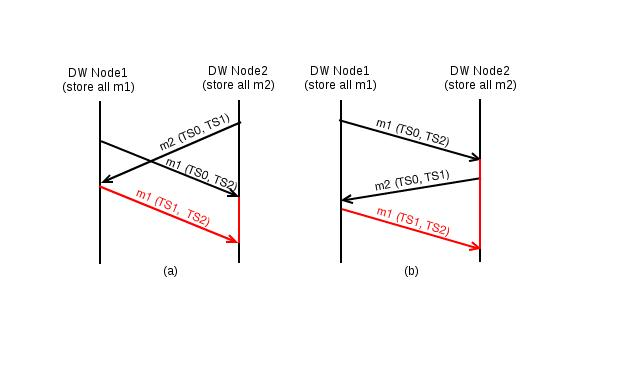
\includegraphics[width=3.3in]{AtomicityOrder.jpg}
\vspace{-18mm}
\caption{Atomicity(a) and Order(b) Violations.}
\label{fig:Atomicity}
\vspace{-5mm}
\end{figure}

However, out-of-order events are expected to occur infrequently. Furthermore, such events are likely to interfere only with a handful of the prior updates. For example, a write on a map followed by an out-of-order read on a different map does not cause a problem.

\subsection{Consistency}

Our system maintains an eventually consistent version of all the maps. The value of the maps may not be consistent at any given moment, but the error is limited to values that have not fully propagated through system. In order to provide consistent version of all the maps, snapshots may be employed at certain points in time, without using a centralized point of synchronization.

Cumulus employs a background task to periodically identify the furthest event in an Introduced Total Order that has been fully propagated. For all the maps, the values set in the most recent TS which logically precedes furthest point TS will be used as consistent version. A period between two consistent version of all the maps is denoted as \textit{epoch}.

Though identifying the furthest point is slow, it does not interfere with any processing nodes normal operations, and can be performed infrequently, for example once every few seconds. The process may begin by sending an EPOCH END from a switch to all other switches. All switches are aware of the DW Nodes they communicated with, so they will send an EPOCH END to each of them. Each DW Node has to provide the last processed TS, but corrective updates has to be taken into account.

DW Nodes must ensure that no further map deltas (corrective updates), regarding an update which logically precedes the last processed TS, will be received after sending the furthest point TS. Using the data flow graph constructed from the WriteLog and the ReadLog, a DW Node could determine the DW Nodes the deltas were sent to. Because this graph is acyclic, deltas could be flushed along it. The process will start from maps/DW Nodes which depends only on input, not on other maps/DW Nodes, and then it will propagate down the graph. After a DW Node ensures no further corrective updates will arrive, it sends EPOCH READY message to the switch containing the last processed TS. In addition, the same message is sent to all the DW Nodes it previously communicated with.

Each switch will compute the minimum TS received from corresponding DW Nodes and forward the TS within EPOCH READY to all other switches. After receiving EPOCH READY from all the other switches, a switch will compute minimum value among them. Once all the switches computed the minimum value, the switches split the work of broadcasting EPOCH COMMIT containing the minimum TS value across the cluster. Once a node receives an EPOCH COMMIT message, it will never again receive an event for a prior epoch.

Our system will provide mechanism to avoid a single switch issues EPOCH END messages all the time. This is easily achieved by a token-passing system and ordering switches. Only the switch with the token can switch epochs. It waits for the duration of one period, switches, and then passes the token to the next switch.

The Log structures grow over time. To prevent unbounded memory usage, we may employ the same background task we used for consistent views to periodically truncate, or garbage collect the entries in each Log structure. The WriteLog and the ReadLog are truncated at this point, and all writes before this point is coalesced into a single entry. The entries from the ReceiveLog which precedes the consistent image TS may be safely deleted. They must not be deleted earlier, since before EPOCH END the corresponding corrective updates may arrive. However, there is an exception from this rule. The ReceiveLog entry may be deleted just after executing a statement if only one map is on the rhs. Nevertheless, for 3 or more joins in the original sql query, there will be multiple maps on the rhs.

Still, a DW Node may run out of memory before the switch with a token switched epochs. In order to avoid this, the DW Node may request end of current EPOCH by sending an EPOCH END REQUEST message to a switch.

As a conclusion, our system will employ a hybrid consistency model, similar to \cite{Bayou95}, in order to provide a user both a low-latency tentative data (the value from the highest TS), or a committed data (a value from the most recent snapshot of the system).

\subsection{Optimizations}
\textbf{Bypass Optimization.} Bypass refers to executing messages on a DW Node in a different order than their TS imply. This is helpful when a message cause DW Node to block and wait for some data to arrive. Thanks to the WriteLog structure, a message received from a switch may bypass an uncompleted PUT message. The PUSH, FETCH and corrective update messages could bypass an uncompleted PUT message if not referring to the same map the uncompleted PUT message is trying to write to. By this restriction, unnecessary corrective updates are avoided.

\textbf{PUT Optimization.} PUT messages sent from a switch to a DW Node may not be used at all. As explained in Section~\ref{Components}, by receiving a PUT message, the DW Write Node will be aware of map update that will be performed upon receiving all the right-hand side maps. However, the DW Write Node will be implicitly notified about map update from a PUSH message. If PUT messages do not exist at all in our system, the ''blind bypassing'' effect is achieved. By blind bypassing, messages will always bypass non-existing PUT message. Since our system could not check restrictions (do not bypass if referring to the same map), corrective updates messages have to be sent. In addition, the WriteLog structure should apply corrective updates as well. If corrective updates eradicated by absence of PUT messages do not cause more traffic than PUT messages themselves, this optimization could reduce network traffic.

\textbf{PUSH Optimization.} On the other side, we could also decrease traffic in network by reducing number of sent PUSH messages. If a map hasn't been updated after last send to particular DW Node, there is no need to send it again. By applying this optimization huge gain is expected, especially when mostly small set of maps is updated. 

The procedure for determining whether a PUSH message will be sent on a FETCH message arrival to a DW Read Node is the following. First, find the most recent TSx of the map prior to FETCH message TS. If the ReadLog structure contains the most recent version of the map, a PUSH message is not sent to to the DW Write Node. For this purpose, the ReadLog structure will additionally contain TSx.

The ReceiveLog structure will suffer from the following changes. Instead of TSy, an entry in the ReceiveLog structure should contain TSx (TS of statement where map got value which was sent). The DW Write Node always use the most recent version of the map prior to TSy.

The DW Write Node could not be aware whether it will receive something from DW Read Node or its current value in the ReceiveLog is the most recent one. Two possibilities may be employed:
\begin{enumerate}[(1)]
 \item Wait for some timeout to give some time for a PUSH messages to arrive, or
 \item Optimistically continue and do corrective updates if the PUSH messages arrive. 
\end{enumerate}

If a switch sends multiple messages per update, the optimization will not work since from multiple PUSH messages per DW Write Node/DW Read Node pair per TS only the first one will be sent. This can be worked around by expanding the ReadLog with the map values. 

\textbf{FETCH Optimization.} It is possible to reduce size of a single FETCH message. If all DW Nodes contain information about map partitioning, a reference to a DW Write Node inside a FETCH message is redundant. However, the system has to inform all DW Nodes in case of map repartitioning.

\textbf{The ReadLog Optimization.} Currently, the ReadLog structure consists of \{map, a reference to DW Node, TS\}. A corrective update message may be applicable to multiple statements from multiple update IDs, so destination need to examine OperationLog in order to check that. Storing multiple TS per single \{map, a reference to DW Node\}, allows a source to point to exact TS on a destination when a corrective update message is sent.

\textbf{Buffering corrective updates.} The system may limit recursive corrective updates by buffering deltas for a short period of time after the corrective update message arrived, allowing multiple subsequent deltas to be aggregated together. We could even deffer corrective updates until the epoch end, or embody the corrective updates with the following PUSH message to the same DW Node.

\textbf{Corrective updates processing.} In order to avoid examining the segment of the OperationLog for each corrective update arrived, a source may send all the TS on destination where a corrective update must be applied. An alternative is to preserve mapping from arrived map to a list of TS on destination where a corrective update may be used. However, this imply slightly more work on a destination.

\textbf{Map compression.} Maps can apply compression techniques to address frequently repeating data.

\textbf{Work-space trade-off. } The system could employ $i$-th order of materialization. Thus, our system amortizes space requirements causing additional work during update.

\textbf{Look ahead.} When the system realizes that some patterns of accessing maps in the Log structures are repeating, prediction of future accesses may be utilized. An approach similar to cache memory may be exploited, so frequently requested maps could be faster accessed. If maps are continuously changing, out system may benefit from prediction of future map updates.

\section{Experiments}
\label{sec:Experiments}
\vspace{2mm}

\section{Related Work}
\label{sec:Related}
\vspace{2mm}

\subsection{Comparison to Transactional Memory}
We will compare our system to a classical Transactional Memory. Here, transactions are implicit at an update level. The order of transactions is defined with TS at the time of the entry in the system (reaching a switch). Our system will execute updates optimistically and store different versions of the data in the WriteLog structure. Instead to aborting and redoing an update, the system may perform the corrective update on the map, if Write-Read dependencies are violated. Since there is no aborts and multiversions are employed, unrecoverable schedules can not arise. Performing periodic garbage collection and consistent snapshot may be regarded as a commit.

A conflict arise if at least two updates:
\begin{enumerate}[(1)]
 \item Execute statements in order not specified via Introduced Total Order, or their execution overlap in time, 
 \item Access same map and
 \item At least one of them performs write.
\end{enumerate}

All of those is detected on per-DW Node basis, since upon receiving a PUT message the ReadLog structure is examined. A conflict is resolved by using corrective updates.

When dealing with any kind of a distributed system, opacity has to be kept in mind. Until now, we discussed serializability of statements (or linearizability of updates). Opacity consists both of serializability and consistent memory view. Any side-effect due to reading values from an inconsistent map is reluctant. Typical examples for this is divide by zero or infinite loops \cite{Rachid08}. Former is not applicable here since only addition and multiplication exist. Later is also not applicable since we do not have loops depending on indexes, only loops over whole domain exist.

\section{Future work}
\label{sec:Future}
\vspace{2mm}

\textbf{Rounds.} We may force our total order by using rounds and enough timeouts between them. For example, after a particular write, reads depending on that write could be postponed for the next round. Still, there is no guaranty corrective updates will never occur, but it will be rare. However, this is hard to implement.

\textbf{Timing assumptions.} Different heuristics can be applied in our system. If an update with significantly lower TS than the DW Node is currently processing have not yet arrived, the DW Node could reasonable suppose it is irrelevant to our DW Node. This heuristic could be based on the estimated message travel time from a switch to a DW Node and the delta query level.

\textbf{Batching.} We only address single-tuple updates in this paper.
Batching and set-at-a-time techniques have often been
very successful in query processing.
We believe that the compilation approach
should remain unchanged -- delta processing with sets of map updates does not
result in code as simple as \M3, while the
execution of \M3 triggers as generated by our current compiler
can easily be batched. We can profit
particularly from batching message content to send fewer messages in
Cumulus runtime.

\textbf{Partitioning.}
Map collections can contain different number of pairs. Collocating corresponding maps (via key-foreign key relationships) of different map collections on the same DW Nodes could significantly decrease network traffic. Database partitioning and co-clustering decisions are traditionally made based on a combination of: 
\begin{enumerate}[(1)]
 \item Workload statistics, 
 \item Information on schema and integrity constraints and
 \item Expert insights into how database execute queries.
\end{enumerate}

Ideally, such decisions should be based on a combination of (1), (2) and data flow analysis. The goal is to decrease total number of messages sent in the system. Using these modifications of data flow dependencies, partitioning and co-clustering decisions can be made by solving a straightforward min-cut style optimization problem. 

In the case of multiple input streams, the probability for data dependency violations and corrective update messages induced is an important factor as well. By a \textit{switch update partitioning}, which refers to an algorithm for assigning updates to switches in some specific order, data dependent events might be executed in secluded points in time. Thus, by tweaking Introduced Total Order, the chances for data dependency violation is lowered.

However, analyzing update streams in order to discover data dependencies and optimize Introduced Total Order is very costly. By the time a long enough sequence of events is collected, computations could already be finished.

Switch update partitioning and data partitioning are dependent on each other. If for a longer period of time a different pattern of updates occurs more frequently, data and a switch update partitioning could be dynamically changed. However, the operation is costly and should be applied very carefully.

\textbf{Redundancy.} Future work will also address using redundant nodes for dealing with node failures. This will also increase availability in the system.

\section{Conclusion}
\label{sec:Conclusion}
\vspace{2mm}

Our preliminary experiments show that the choices made in our
system indeed allow us to realize the embarrassing parallelism and
thus the scalability in a cluster that is promised by our approach of
compiling to M3 programs.  We showed that the our system infrastructure scales linearly, both in terms of updates and client queries, with the number of nodes in the system.

The system we implemented avoids locks, but price is payed for preserving multiple map versions. The processing nodes never waits for the map, but the system compensates it using the corrective updates. We saw that all the dependency violations can be fixed by corrective updates, which does not significantly degrade performance. In most cases, corrective updates will not occur too frequently. That mechanism will enable us to elude building our implementation based on some special and expensive network features.

{
\bibliographystyle{abbrv}
\bibliography{refs,main}
}

\newpage

\end{document}